%%%%%%%%%%%%%%%%%%%%%%%%%%%%%%%%%%%%%%%%%%%%%%%%%%%%%%%%%%%%%%%%%
% Projeto avaliativo da disciplina de programação 2
% Sub-projeto do grupo Doyle
%
% Autores:
%     Prof. Dr. Ruben Carlo Benante
%
%     Guilherme Rodrigues Chaves Do Nascimento
%     Thiago De Azevedo Cavendish
%     Mateus Simplicio De Barros
%     Ulisses Mosart Sobrinho
%     Joao Alves Pereira Neto
%     Maria Isabel Do Nascimento Freitas
%
% Data: 2021-11-08
%
% Assunto: escrever uma linha de explicação: Aulas sobre estruturas de controle de decisão
%
%%%%%%%%%%%%%%%%%%%%%%%%%%%%%%%%%%%%%%%%%%%%%%%%%%%%%%%%%%%%%%%%%

           % Geraçao do PDF %
%%%%%%%%%%%%%%%%%%%%%%%%%%%%%%%%%%%%%%%%%%%%%%%%%%%%%%%%%%%%%%%%%
% Para gerar o PDF use uma das 2 opções abaixo:
%
% Opção 1: com makefile
%    $ make pext-prog2-benante-sobrenome1-sobrenome2*.pdf
%
% Opção 2: comandos diretos:
%    $ pdflatex pext-matdiscreta-benante-sobrenome1-sobrenome2.tex -o pext-matdiscreta-benante-sobrenome1-sobrenome2.pdf
%    $ bibtex biblio 
%    $ pdflatex pext-matdiscreta-benante-sobrenome1-sobrenome2.tex -o pext-matdiscreta-benante-sobrenome1-sobrenome2.pdf

% preambulo %%%%%%%%%%%%%%%%%%%%%%%%%%%%%%%%%%%%%%%%%%%%%%%%%%%%%%
\documentclass[a4paper,12pt]{article}  % Duas colunas
\usepackage[utf8]{inputenc}  % letras acentuadas
\usepackage[portuguese]{babel}  % tradução de títulos
\usepackage{algorithm}  % ambiente para índice de algoritmos
\usepackage{algpseudocode}  % fonte e estilo do algoritmo
\usepackage{graphicx}
\usepackage{indentfirst}
% \usepackage{natbib}
%[noend]

\floatname{algorithm}{Algoritmo} % tradução da palavra algorítimo no ambiente de índice

%% Capa %%%%%%%%%%%%%%%%%%%%%%%%%%%%%%%%%%%%%%%%%%%%%%%%%%%%%%

\begin{document} % início do PDF %

\begin{center}
    \vspace{-30mm}
    \LARGE{ESCOLA POLITÉCNICA DE PERNAMBUCO}
    \vspace{10mm}
    \\ \LARGE{Programação 2:
Aulas sobre estruturas de controle de decisão}
    \vspace{30mm}
    \\ \large{Ruben Carlo Benante \\ Guilherme Rodrigues Chaves Do Nascimento \\ Thiago De Azevedo
Cavendish \\ Mateus Simplicio De Barros \\ Ulisses Mosart Sobrinho \\ Joao Alves Pereira Neto \\ Maria Isabel Do Nascimento Freitas}
    \vspace{60mm}
    \\ \large{8 de novembro de 2021}
\end{center}

%% Resumo %%%%%%%%%%%%%%%%%%%%%%%%%%%%%%%%%%%%%%%%%%%%%%%%%%%%%%

\newpage

\begin{abstract}

\textbf{Assunto:} Ensino de estruturas de controle de decisão, da Linguagem de Programação \texttt{C}.

 Vamos comparar os algoritmos de estruturas de controle de decisão % \textit{xsort} e \textit{ysort} para bla bla.
% descrever em poucas palavras seu projeto aqui 

\textbf{Local:} Escola Politécnica de Pernambuco - UPE/POLI

\textbf{Órgão Financiador:} N/A

\textbf{Caracterização:} Projeto requisito da disciplina de Programação 2, sub-projeto do grupo \texttt{Doyle}

\end{abstract}

%% Sumário %%%%%%%%%%%%%%%%%%%%%%%%%%%%%%%%%%%%%%%%%%%%%%%%%%%%%

\newpage

\tableofcontents

% Artigos %%%%%%%%%%%%%%%%%%%%%%%%%%%%%%%%%%%%%%%%%%%%%%%%%%%%%%

%% seção de introdução %%%%%%%%%%%%%%%%%%%%%%%%%%%%%%%%%%%%%%%%%

\newpage

\section{Introdução}

% Descrever melhor seu projeto aqui 

   Esse projeto será composto de duas vídeo aulas sobre o tópico de ensino de estruturas de controle de decisão,  da Linguagem de Programação \texttt{C}

\begin{itemize}

 \item Estrutura de decisão If/Else
 \item Estrutura de controle Switch
\end{itemize}


 \subsection{Função básica}
% As estruturas de decisão If/Else tem como principal função ...


    Nós utilizamos as estruturas de decisão (If/Else) quando existem instruções
dentro do programa que só devem ser executadas se elas satisfizerem  
determinadas condições. \newline

Por exemplo :

\begin{itemize}
               
       \item  Só irei para a praia se não chover. 
       \item  Só passarei nesta disciplina se eu obtiver uma média igual ou superior a 7,0 e se a presença for superior ou igual a 70 \% das aulas.
             
\end{itemize}

   - A sintaxe da estrutura IF na linguagem C é a seguinte :
 
 \subsection{Estrutura de Decisão IF}   
       
  -  Comando IF = se
   
  \\
\begin{table}[H]
\begin{center}
 \caption{Tabela para melhor vizualização da estrutura do If}
\begin{tabular}{|l|r|}
  \hline \hline
  
  .          & if(condição) \\ \hline
  Estrutura  &  \{           \\ \hline
    básica   &   lista de instruções  \\ \hline
  .          &  \}             \\ \hline
  
\end{tabular}
\label{tab:resultados}
\end{center}
\end{table}


  O algoritmo \textit{acima} trabalha da seguinte maneira :
 \\

  -  A condição é verificada a cada passagem pela estrutura IF. Se a condição for satisfeita (V), então a lista de instruções que se encontra entre chaves será executada. \newline
   
  Porém, Se a condição NÃO for satisfeita (F), então serão executadas as instruções existentes logo após o fechamento das chaves.
 
 \subsection{Else}
 \subsubsection{Sobre} % a ser ajustado o nome dessa sessao 

   Podemos pensar no comando else como sendo um complemento do comando if, sendo possível associar um else com qualquer if. Se a expressão condicional associada a if é verdadeira, o bloco de instruções associada será executado. \newline 

   Se for falsa, então o bloco de instruções do else será executado, assim que uma condição verdadeira é encontrada, o bloco associado a ela será executado, e o resto do encadeamento é ignorado. \newline 
Se nenhuma das condições for verdadeira, então o else final será executado.

  
 \subsection{Switch}
 \subsubsection{Sobre} % a ser ajustado o nome dessa sessao
    
   A palavra switch, associando ao seu significado do inglês, é um comando que funciona como uma chave de seleção/interruptor, sendo capaz de acionar tanto uma como diversas escolhas. \newline
   
   O switch case é um comando utilizado na construção de menus de escolhas(“cases”) para o usuário, o qual diante de um leque de opções, poderá decidir algum dos casos e assim obter uma resposta relativa ao caso selecionado.
 

  \subsubsection{Aplicações}
 % \subsubsection{Primeira aplicação}

   O comando “switch(variável)” assemelha seu funcionamento a de conjuntos “if-else”, como demonstrado logo abaixo em um programa cuja principal finalidade é receber e atribuir valores para a variável “valor” e em seguida imprimir na tela uma resposta de acordo com o valor digitado: 

 \begin{figure}[H]
 \centering
 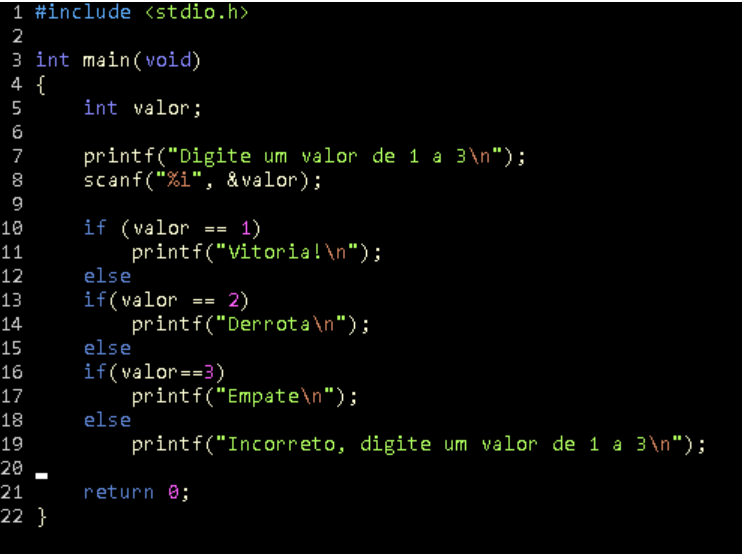
\includegraphics[width=.80\linewidth]{imagens/ex2.png}
 \caption{Exemplo de programa com alguns conjuntos de if-else}
 \label{fig:xsorta}
\end{figure}

   Assim como demonstrado acima, é possível criar uma sequência “if-else” em cadeia gerando um conjunto de casos que terão a mesma eficiência do comando switch, no entanto, caso o menu necessite diversos casos, o programa provavelmente ficará desorganizado e estará ocupando bastante espaço de maneira desnecessária. \par
   
\\
  
   Agora, apresentando o mesmo programa, só que aplicando o conceito de “switch-case”, ficaria da seguinte maneira:

\begin{figure}[H]
 \centering
 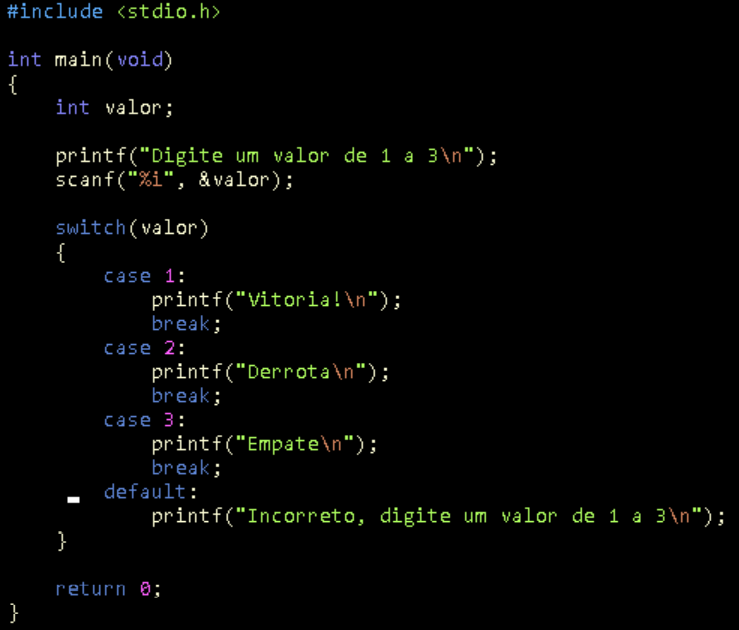
\includegraphics[width=.80\linewidth]{imagens/ex3.png}
 \caption{Aplicando o switch ao invés do if-else}
\end{figure}


 %\subsubsection{Segunda aplicação}

   Assim como o “if-else”, switch pode receber tanto um inteiro ou caractere como variável, exemplificado no programa a seguir:

\begin{figure}[H]
 \centering
 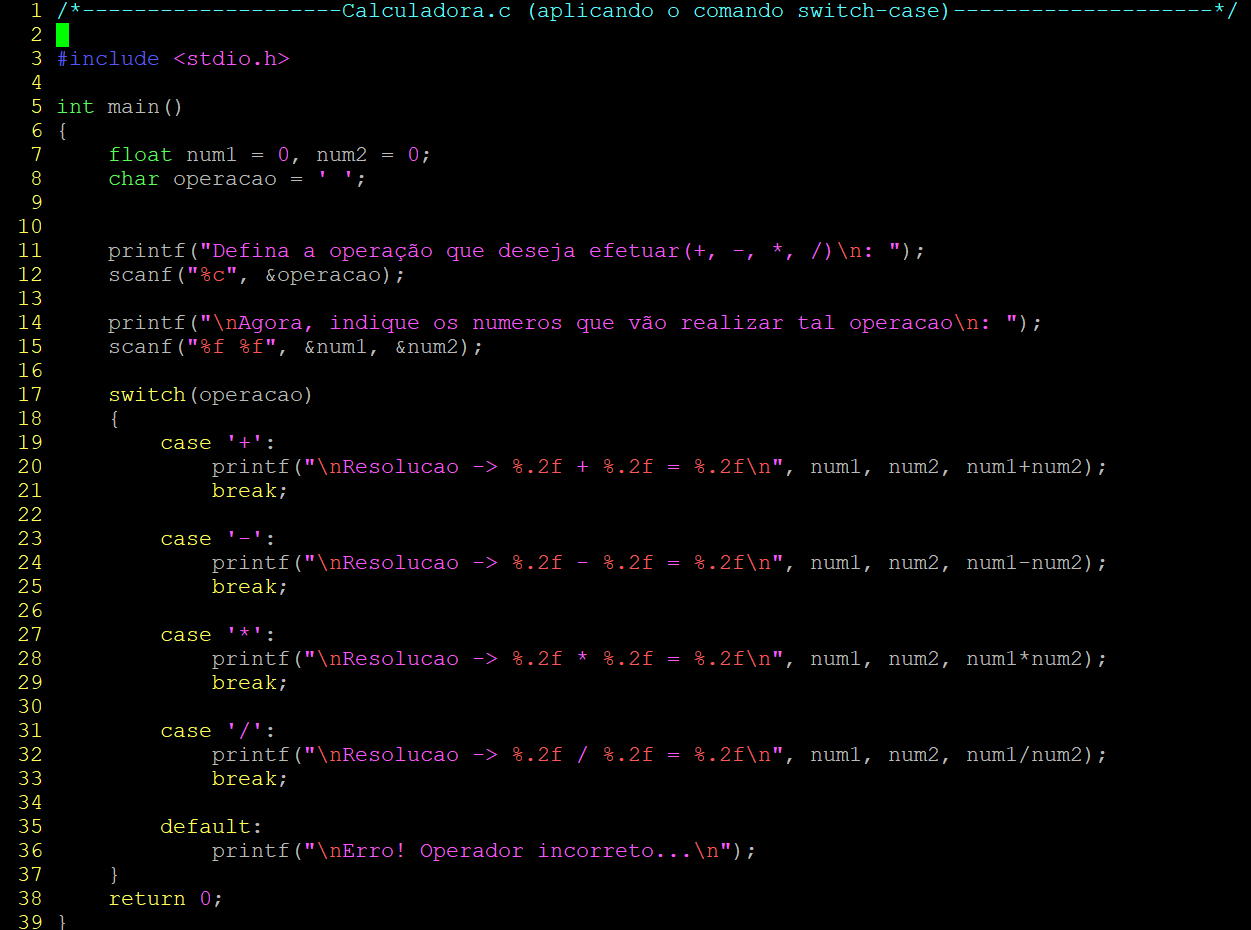
\includegraphics[width=.80\linewidth]{imagens/ex4.png}
 \caption{Calculadora} %fique a vontade para alterar o nome da imagem guilherme
 \label{fig:xsort}
\end{figure}

   O programa aproveita da praticidade do comando “switch(variável)”, simplificando toda a complexidade que necessitária de vários “if...else” encadeados. \par
 Nessa calculadora, o usuário deverá digitar a operação seguida dos números a fim de realizar o cálculo em questão: 
 
 \begin{figure}[H]
 \centering
 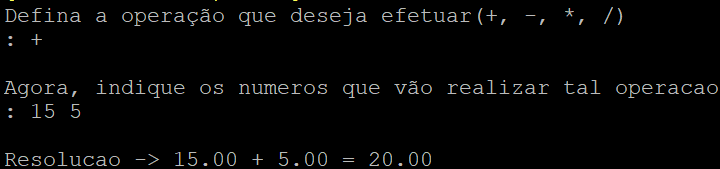
\includegraphics[width=.80\linewidth]{imagens/ex5.png}
 \caption{Operação de soma}
 \end{figure}

 \begin{figure}[H]
 \centering
 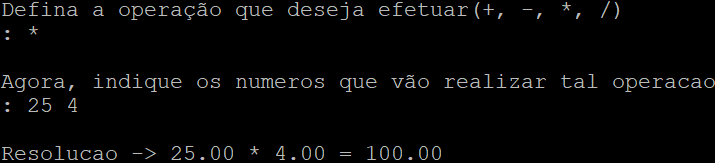
\includegraphics[width=.80\linewidth]{imagens/ex6.png}
 \caption{Operação de multiplicação}
\end{figure}

     A instrução “break” no código termina a execução do switch, evitando testar os demais comandos possíveis de forma desnecessária. \par
   \\
     O comando “default” serve para exibir uma mensagem caso nenhuma das operações anteriores tenham sido devidamente declaradas:


 \begin{figure}[H]
 \centering
 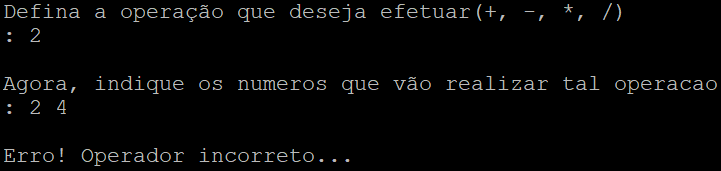
\includegraphics[width=.80\linewidth]{imagens/ex7.png}
 \caption{Operação indefinida}
\end{figure}


%% seção de objetivos %%%%%%%%%%%%%%%%%%%%%%%%%%%%%%%%%%%%%%%%%%%%%%%%%%%%%%
\section{Objetivos}

 \subsection{Objetivo Geral}

  O projeto tem como objetivo, lecionar sobre as estruturas condicionais da linguagem de programação C, tal como sua utilização pratica em código. 

 \subsection{Objetivos Específicos}

\begin{itemize}
 \item Lecionar sobre os tipos de estruturas condicionais da linguagem de programação C.
 \item Lecionar sobre a implementação das estruturas de forma pratica em um código, buscando o aprendizado dinâmico.  
\end{itemize}


%% seção de justificativa %%%%%%%%%%%%%%%%%%%%%%%%%%%%%%%%%%%%%%%%%%%%%%%%%%%%%%
\section{Justificativa}

 

%\begin{figure}[ht]
%\centering
%\includegraphics[width=.80\linewidth]{imagens/exemplo.png}
%\caption{Exemplo de ordenação com Bubblesort}
%\label{fig:xsort}
%\end{figure}


%% seção de metodologia %%%%%%%%%%%%%%%%%%%%%%%%%%%%%%%%%%%%%%%%%%%%%%%%%%%%%%
\section{Metodologia}

    O projeto será composto de duas vídeo aulas sobre as estruturas condicionais da linguagem de programação \texttt{C}.

\begin{itemize}

 \item Aula sobre as estruturas de decisão If e Else.
 \item Aula sobre a estrutura de controle Switch.

\end{itemize}



 % subseção equipamentos %%%%%%%%%%%%%%%%%%%%%%%%%%%%%%%%%%%%%%%%%%%%%%%%%%%%%%
 \subsection{Equipamentos Necessários}

% Listar os equipamentos necessários para a implementação do projeto.

   Para realizar este projeto é preciso ter um computador ou um meio de acesso a uma IDE, como por exemple a (coding C) para Android, também é necessário tem acesso à internet e disponibilidade para assistir as vídeo aulas gravadas.


 % O método \emph{Ysort} é caracterizado por...

 % subseção com algoritmo %%%%%%%%%%%%%%%%%%%%%%%%%%%%%%%%%%%%%%%%%%%%%%%%%%%%%%
 \subsection{Implementação}

   A implementação será feita por meio do compartilhamento de playlist em um ambiente que será escolhido pelo orientador Doutor professor Ruben Carlo Benante.



% O algoritmo \textit{Ysort} segue abaixo:   %%%%%% Configuração de jogo %%%%%%

%\begin{algorithm}
%\caption{Algoritmo Ysort}\label{alg:ysort}
%\begin{algorithmic}[1]
%\Function{ysort}{estado}\Comment{retorna uma ação}
%\State \textbf{Entradas}: estado é a configuração atual do jogo
%\State $v\gets \mathrm{maxvalor}{(estado)}$
%\State \textbf{returna} a ação $a$ em sucessores(estado) cujo valor é $v$ %\Comment{comentario}
% \While{$r\not=0$}\Comment{We have the answer if r is 0}
% \State $a\gets b$
% \State $b\gets r$
% \State $r\gets a\bmod b$
% \EndWhile\label{euclidendwhile}
%\EndFunction
%\Function{maxvalor}{estado}\Comment{retorna o valor estático}
%\If{fim(estado)}
%   \State \textbf{retorna} estatico(estado)
%\EndIf
%\State $v \gets -\infty$
%\For{todas ações $a$ nos sucessores(estado)}
%    \State $v \gets \max{(v, \mathrm{minvalor}(a))}$
%\EndFor
%\State \textbf{retorna} $v$
%\EndFunction
%\Function{minvalor}{estado}\Comment{retorna o valor estático}
%\If{fim(estado)}
%   \State \textbf{retorna} estatico(estado)
%\EndIf
%\State $v \gets \infty$
%\For{todas ações $a$ nos sucessores(estado)}
%    \State $v \gets \min{(v, \mathrm{maxvalor}(a))}$
%\EndFor
%\State \textbf{retorna} $v$
%\EndFunction
%\end{algorithmic}
%\end{algorithm}


%% seção Plano de Trabalho %%%%%%%%%%%%%%%%%%%%%%%%%%%%%%%%%%%%%%%%%%%%%%%%%%%%%%
\section{Plano de Trabalho}

     Etapa 1: Organização inicial.
    \begin{itemize}
        \item Divisão de trabalhos.
        \item Pesquisa.
        \item Implementações no PDF.
    \end{itemize}
     Etapa 2: Planejamento estratégico.
    \begin{itemize}
        \item Planejamento do Roteiro.
        \item Metodologia das aulas.
        \item Criação dos códigos para as aulas.
    \end{itemize}
     Etapa 3: Criação e ajustes dos códigos para as aulas.
    \begin{itemize}
        \item Finalização dos códigos para as aulas.
        \item Ajustes finais (pré-gravação).
        \item Término do PDF.
    \end{itemize}
     Etapa 4: Finalização..
    \begin{itemize}
        \item Revisão.
        \item Roteiro.
        \item Gravação dos vídeos.
        \item Edição dos vídeos.
    \end{itemize}

% seção Plano de Trabalho / Cronograma %%%%%%%%%%%%%%%%%%%%%%%%%%%%%%%%%%%%%%%%%%%%%%%%%%%%%%
\section{Cronograma}

   Em conjunto com a seção de Plano de Trabalho, a seção de cronograma coloca as atividades dispostas numa linha do tempo.


   Utilize uma tabela para melhor visualização.

\begin{table}[H]
\begin{center}
 \caption{Relação etapas - organização diária}
\begin{tabular}{|l|r|}
  \hline \hline
  Etapas & Dias  \\ \hline 
  1- Organização inicial &  20/10 - 27/10  \\ \hline
  2- Planejamento estratégico & 27/10 - 30/10 \\ \hline
  3- Criação e ajustes  &  31/10 - 05/11 \\ \hline
  4- Finalização & 05/11 - 07/11 \\ \hline
\end{tabular} 
%\label{tab:resultados}
\end{center}
\end{table}

%% seção de impactos alcançados %%%%%%%%%%%%%%%%%%%%%%%%%%%%%%%%%%%%%%%%%%%%%%%%%%%%%%
\section{Impactos alcançados } % e Transferências

 % subseção de impacto científico %%%%%%%%%%%%%%%%%%%%%%%%%%%%%%%%%%%%%%%%%%%%%%%%%%%%%%
 \subsection{Impacto Científico}

  Não há impacto científico relevante.

 % subseção de impacto tecnológico %%%%%%%%%%%%%%%%%%%%%%%%%%%%%%%%%%%%%%%%%%%%%%%%%%%%%%
 \subsection{Impacto Tecnológico}

   Não há impacto tecnológico relevante.

 % subseção de econônimo %%%%%%%%%%%%%%%%%%%%%%%%%%%%%%%%%%%%%%%%%%%%%%%%%%%%%%
 \subsection{Impacto Econômico}

   Esse projeto não tem nenhum interesse econômico.

 % subseção de impacto social %%%%%%%%%%%%%%%%%%%%%%%%%%%%%%%%%%%%%%%%%%%%%%%%%%%%
 \subsection{Impacto Social}

   O projeto visa contribuir com o aprendizado das futuras geraçoes da sociedade de forma que ajude a democratizar o conhecimente por intermédio de uma plataforma de compartilhamento de vídeos.


 % subseção de impacto ambiental %%%%%%%%%%%%%%%%%%%%%%%%%%%%%%%%%%%%%%%%%%%%%%%%%%%%%%

%% seção de Conclusão %%%%%%%%%%%%%%%%%%%%%%%%%%%%%%%%%%%%%%%%%%%%%%%%%%%%%%%%%%%%
\section{Conclusão}

   -  O Grupo Doyle terá como objetivo na execução dessas aulas ensinar o controle de decisão, da linguagem C, aos discentes interessados.
 Contará com sua exposição de ensino gravada, que será disponibilizada e sua elaboração, a fim de cumprir com os aspectos estabelecidos no Plano de Trabalho.

 % subconclusão %%%%%%%%%%%%%%%%%%%%%%%%%%%%%%%%%%%%%%%%%%%%%%%%%
%%%%%
% \subsection{Concluindo}


 % O que mais o seu projeto agrega? O que é transferido? De onde vem? Para onde vai?


%% seção de resultados esperados %%%%%%%%%%%%%%%%%%%%%%%%%%%%%%%%%%%%%%%%%%%%%%%%%%%%%%
\section{Resultados Esperados}

%  Os resultados mostrados na tabela \ref{tab:resultados} demonstram ...


   Concluimos, para fins educacionais, que a estrutura de decisão switch é a mais indicada entre as estruturas condicionais apresentadas, se tratando de diversas situações,  por causa da sua praticidade de trabalhar em códigos mais compactos e eficientes. \newline


   - De acordo com \cite{benante2008phd} e este é o fim do artigo.


%%%%%%%%%%%%%%%%%%%%%%%%%%%%%%%%%%%%%%%%%%%%%%%%%%%%%%%%%%%%%%%%%%%%%%%%%%%%%%%%%%%%%%%%%%%%%%%%%%%%%%%%%%%%
% referências bibliográficas %%%%%%%%%%%%%%%%%%%%%%%%%%%%%%%%%%%%%%%%%%%%%%%%%%%%%%
\section{Referências Bibliográficas}

% cite todos, mesmo os não referenciados %%%%%%%%%%%%%%%%%%%%%%%%%%%%%%%%%%%%%%%%%%%%%%%%%%%%%%
\nocite{*}

% se necessario %%%%%%%%%%%%%%%%%%%%%%%%%%%%%%%%%%%%%%%%%%%%%%%%%%%%%%
% troca autor and autor por autor & autor, na bibliografia. O dcu usa "and"
%\renewcommand{\harvardand}{\&} % troca and pro &. O dcu usa "and"

% Estilos de bibliografia %%%%%%%%%%%%%%%%%%%%%%%%%%%%%%%%%%%%%%%%%%%%%%%%%%%%%%
% \bibliographystyle{abnt-alf} % Estilo alfabético da ABNT. Opção [num] para estilo numérico
%\bibliographystyle{apalike}
%\bibliographystyle{dcu} %citacao como (autor and autor, ano). Parece apalike. Rev. Control. Automacao. Use com harvard
%\bibliographystyle{agsm} % padrao harvard fica (autor & autor ano).
\bibliographystyle{acm}

% arquivo de banco de dados das referências %%%%%%%%%%%%%%%%%%%%%%%%%%%%%%%%%%%%%%%%%%%%%%%%%%%%%%
% renomear para o número do exercício correto
% o arquivo de bibliografia pode se chamar qualquer coisa, isso não muda o comando de gerar o PDF. 
% Por exemplo para 'mybiblio.bib', use \bibliography{mybiblio} e os comandos pdflatex e bibtex continuam os mesmos identicos com exN.
\bibliography{biblio}

\end{document}
